\documentclass[12pt]{article}\usepackage[]{graphicx}\usepackage[]{color}
%% maxwidth is the original width if it is less than linewidth
%% otherwise use linewidth (to make sure the graphics do not exceed the margin)
\makeatletter
\def\maxwidth{ %
  \ifdim\Gin@nat@width>\linewidth
    \linewidth
  \else
    \Gin@nat@width
  \fi
}
\makeatother

\definecolor{fgcolor}{rgb}{0.345, 0.345, 0.345}
\newcommand{\hlnum}[1]{\textcolor[rgb]{0.686,0.059,0.569}{#1}}%
\newcommand{\hlstr}[1]{\textcolor[rgb]{0.192,0.494,0.8}{#1}}%
\newcommand{\hlcom}[1]{\textcolor[rgb]{0.678,0.584,0.686}{\textit{#1}}}%
\newcommand{\hlopt}[1]{\textcolor[rgb]{0,0,0}{#1}}%
\newcommand{\hlstd}[1]{\textcolor[rgb]{0.345,0.345,0.345}{#1}}%
\newcommand{\hlkwa}[1]{\textcolor[rgb]{0.161,0.373,0.58}{\textbf{#1}}}%
\newcommand{\hlkwb}[1]{\textcolor[rgb]{0.69,0.353,0.396}{#1}}%
\newcommand{\hlkwc}[1]{\textcolor[rgb]{0.333,0.667,0.333}{#1}}%
\newcommand{\hlkwd}[1]{\textcolor[rgb]{0.737,0.353,0.396}{\textbf{#1}}}%

\usepackage{framed}
\makeatletter
\newenvironment{kframe}{%
 \def\at@end@of@kframe{}%
 \ifinner\ifhmode%
  \def\at@end@of@kframe{\end{minipage}}%
  \begin{minipage}{\columnwidth}%
 \fi\fi%
 \def\FrameCommand##1{\hskip\@totalleftmargin \hskip-\fboxsep
 \colorbox{shadecolor}{##1}\hskip-\fboxsep
     % There is no \\@totalrightmargin, so:
     \hskip-\linewidth \hskip-\@totalleftmargin \hskip\columnwidth}%
 \MakeFramed {\advance\hsize-\width
   \@totalleftmargin\z@ \linewidth\hsize
   \@setminipage}}%
 {\par\unskip\endMakeFramed%
 \at@end@of@kframe}
\makeatother

\definecolor{shadecolor}{rgb}{.97, .97, .97}
\definecolor{messagecolor}{rgb}{0, 0, 0}
\definecolor{warningcolor}{rgb}{1, 0, 1}
\definecolor{errorcolor}{rgb}{1, 0, 0}
\newenvironment{knitrout}{}{} % an empty environment to be redefined in TeX

\usepackage{alltt}
\usepackage[utf8]{inputenc}
\usepackage{graphicx}
\usepackage{float}

\usepackage{amssymb,amsmath}
\usepackage{enumerate}
\usepackage{float}
\usepackage{verbatim}
\usepackage{setspace}
\usepackage{multicol}


\setlength{\textwidth}{6.5in}
\setlength{\textheight}{9in}
\setlength{\oddsidemargin}{0in}
\setlength{\evensidemargin}{0in}
\setlength{\topmargin}{-1.5cm}
\setlength{\maxwidth}{6.5in}

\title{\vspace{-2.0cm} Stat 532 Project: Statistical arrival models to estimate missed passage counts at fish weirs}
\author{By Suresh Andrew Sethi and Catherine Bradley, Project by Leslie Gains-Germain}
\date{Fall 2015}
\IfFileExists{upquote.sty}{\usepackage{upquote}}{}
\begin{document}


\maketitle
\tableofcontents

\newpage

\section{Introduction}

The goal of this paper is to provide a new method for imputing passage counts on missed dates when enumerating fish passing by a weir. A weir is a device, pictured below, designed to span an entire stream and count every single fish that passes by. 

\begin{center}
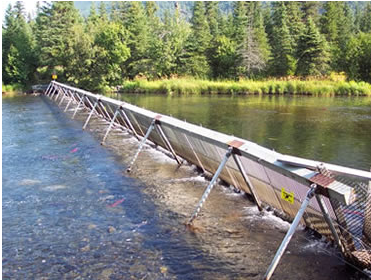
\includegraphics[scale=0.5]{weir.png}
\end{center}

\noindent Weirs do not always operate as intended, however. High water can destroy a weir, bears can interfere with the weir or the weir operator, and ice can delay the installation or require early removal of a weir. \\

\noindent Sethi and Bradley explain that the current method used to impute passage counts on missing dates ``typically involve a ``connect-the-dots'' linear interpolation scheme (e.g. Gewin et al. 2005; Johnson et al. 2007)''. They explain that while this method is easy to implement, it has two main drawbacks. First, it does not provide uncertainty in the missing passage estimates, and second it cannot estimate missing dates at the beginning and end of the run. \\

\noindent The methods proposed by Sethi and Bradley in this paper solve both of these drawbacks. They use a parametric curve to describe the passage of a run of fish at a weir (referred to as the arrival model), and a separate probability model to describe the variability of fish counts around the run curve. The following quote is a nice summary of their reasons for using Bayesian implementation.
\begin{quote}
Models are fit in a Bayesian framework, providing a straightforward means to summarize uncertainty about total run size estimates, arrival model characteristics (e.g. peak run date), and estimates of predicted passage counts on missing-observation dates (Sethi and Bradley 5).
\end{quote}

\noindent The main research goal is to provide a new method for estimating total run size and missed passage counts. The secondary research goal is to estimate parameters of the arrival model that describe the passage of fish over time.


\section{Model}

First, they specify the run curves, or arrival models, that describe the passage of fish over time at a weir. They use two common cumulative distribution functions to describe the run curves, the normal distribution and the skew normal distribution. It is important to note that they could have used any parametric curve for this purpose, but they chose common cumulative distribution functions for convenience. The following quote provides a nice concise explanation.
\begin{quote}
To avoid confusion, it is worth emphasizing that the cumulative distribution functions used to specify arrival dynamics do not represent probability models for weir passage counts; they are merely convenient mathematical functions to describe the shape of the arrival curve of fish at a weir (Sethi and Bradley 8).
\end{quote}

\noindent Below, I use the same notation they use in the paper because I think it's really clear. \\

{\bf Normal Run Curve}  \hfill $p_t = F_N(\mu, \sigma) = \frac{1}{\sigma\sqrt{2\pi}} \int_{-\infty}^t e^{\frac{-(\nu - \mu)^2}{2\sigma^2}}d\nu$ \\

{\bf Skew Normal Run Curve} \hfill $p_t = F_{SN}(t|\xi, \omega, \alpha) = \frac{2}{\omega}\phi(\frac{t-\xi}{\omega}) \Phi(\frac{\alpha(t-\xi)}{\omega})$ \\

\noindent where $p_t$ is the cumulative proportion of the run that has passed the weir at time step $t$. A time step $t$ is defined as a $24$ hour day because daily counts are commonly recorded as weir data. \\

\noindent $F_N$ and $F_{SN}$ are the cumulative distribution functions for the normal and skew normal distributions, respectively. $\mu$ and $\sigma$ are the location and scale parameters for the normal model. For the skew normal model, $\xi$ is the location parameter, $\omega$ is the scale parameter, and $\alpha$ is the shape parameter. $\phi$ is the standard normal density function and $\Phi$ is the standard normal cumulative distribution function.\\

\noindent Daily passage counts are calculated as follows.

$$c_t = S(p_t - p_{t-1})$$

\noindent where $c_t$ is a daily passage count for a given run curve and $S$ is the total run size scalar. \\

\noindent Below are the priors for the parameters of the normal run curve:
\begin{align*}
\mu &\sim Unif(150, 300) \hspace{2in} f(\mu) = \frac{1}{150} I(\mu)_{(150, 300)} \\
\sigma &\sim Unif(1, 50) \hspace{2in} f(\sigma) = \frac{1}{49} I(\sigma)_{(1, 50)} \\
log(S) &\sim N(7.5, 0.25) \hspace{2in} 
f(log(S)) = \frac{1}{\sqrt{0.125\pi}}e^{-\frac{(log(S)-7.5)}{0.125}}  
\end{align*}

\noindent Below are the priors for the parameters of the skew-normal run curve:
\begin{align*}
\xi &\sim Unif(150, 300) \hspace{2in} f(\xi) = \frac{1}{150} I(\xi)_{(150, 300)} \\
\omega &\sim Unif(1, 50) \hspace{2in} f(\omega) = \frac{1}{49} I(\omega)_{(1, 50)} \\
\alpha &\sim Unif(-10, 10) \hspace{2in} f(\alpha) = \frac{1}{20} I(\alpha)_{(-10, 10)} \\
log(S) &\sim N(7.5, 0.25) \hspace{2in} 
f(log(S)) = \frac{1}{\sqrt{0.125\pi}}e^{-\frac{(log(S)-7.5)}{0.125}}  
\end{align*}

\noindent Next, a probability model is used to describe the amount of variation in the passage counts around the run curve. \\

{\bf Normal Process Variation}  \hfill  $c_t^0 \sim N(c_t, \tau)$ \\

{\bf Negative Binomial Process Variation} \hfill $c_t^0 \sim NegBinom(\lambda = \frac{\theta}{\theta + c_t}, \theta)$ \\

\noindent where $c_t^0$ is an observed passage count, $\tau$ is the variance of the normal model, and $\theta$ is the dispersion parameter of the negative binomial model. \\

\noindent Below are the priors for the parameters of the normal process variation model:
\begin{align*}
\tau &\sim Unif(0.1, 1000) \hspace{2in} f(\tau) = \frac{1}{999.9} I(\tau)_{(0.1, 1000)} 
\end{align*}

\noindent Below are the priors for the parameters of the negative binomial process variation model:
\begin{align*}
\theta &\sim Gam(0.1, 0.1) \hspace{2in} f(\theta) = \frac{\theta^{-0.9}0.1^{0.1}e^{-0.1\theta}}{\Gamma(0.1)}
\end{align*}

%% talk about shapes of each run curve and error model and what they mean, and how they incorporate prior knowledge

%% talk about choice of priors for each

\section{Simulation of artificial data}

I started by writing my own code to simulate data. During the process, I realized that code for simulating data is included in the paper. I compared my code to the code they used for simulations, and I decided to show their code here (cleaned up a little bit by me) and include a thorough description of what they did. It was pretty similar to the code I wrote, but sometimes I learn more by going through someone else's code than I do from writing my own code, especially having first written it myself. \\

\noindent They started by defining the skew normal run curve. The location parameter of the skew normal run curve ($\xi$) was set at $185$ because sets the run peak to occur around the $4$th of July. The scale parameter ($\omega$) was set at $7.5$ because this produces a run of about two months long. This makes sense, because salmon usually run up the river in the summer, and the run usually lasts about two months. The skew parameter ($\alpha$) was set to $0$ in the simulations. The total run size was set at $10000$ fish.\\

They used the \verb+psn+ function in the \verb+sn+ package to define the skew normal run curve. After defining the passage counts for each day according to the run curve, they simulated observed passage counts by taking random draws from a negative binomial distribution centered at the run curve with dispersion parameter equal to $7$. The overdispersion parameter was set to $7$ and ``was chosen to reflect variation observed in actual Yukon River Pacific Salmon data (Sethi and Bradley $12$).''

\begin{knitrout}\footnotesize
\definecolor{shadecolor}{rgb}{0.969, 0.969, 0.969}\color{fgcolor}\begin{kframe}
\begin{alltt}
\hlcom{#Simulate "true" data modeled after Pacific Salmon runs: Normal arrival curve model, }
\hlcom{#run size = 10,000 fish,}
\hlcom{#negative binomial process error}
\hlkwd{set.seed}\hlstd{(}\hlnum{205}\hlstd{)} \hlcom{# set random seed if desired}

\hlcom{# Normal-curve shaped arrival model parameters}
\hlstd{true.day.v} \hlkwb{<-} \hlnum{1}\hlopt{:}\hlnum{365} \hlcom{# model time steps, modeled as 24 hour days, e.g. Julian days}
\hlstd{skew} \hlkwb{<-} \hlnum{0} \hlcom{# force skew to zero}
\hlstd{run.mu} \hlkwb{<-} \hlnum{185} \hlcom{# results in a mode on approximately 4th of July peak run}
\hlstd{run.sd} \hlkwb{<-} \hlnum{7.5} \hlcom{# produces a run of about 40 days long}
\hlstd{S} \hlkwb{<-} \hlnum{10000} \hlcom{# 10k fish run}

\hlcom{#Negative Binomial variation parameter}
\hlstd{theta} \hlkwb{<-} \hlnum{7.0} \hlcom{#overdispersion based on Pacific salmon data}

\hlcom{# simulate run arrival under the arrival model}
\hlcom{# for convenience the sn package is used, defining a skewnormal with shape = 0, }
\hlcom{#i.e. Normal distribution}
\hlkwd{require}\hlstd{(sn)}
\hlstd{true.run.v} \hlkwb{<-} \hlstd{S}\hlopt{*}\hlstd{(}\hlkwd{psn}\hlstd{(true.day.v,} \hlkwc{xi} \hlstd{= run.mu,} \hlkwc{omega} \hlstd{= run.sd,} \hlkwc{alpha} \hlstd{= skew,}
                     \hlkwc{engine} \hlstd{=} \hlstr{"biv.nt.prob"}\hlstd{)}
                 \hlopt{-} \hlkwd{psn}\hlstd{(true.day.v} \hlopt{-} \hlnum{1}\hlstd{,} \hlkwc{xi} \hlstd{= run.mu,} \hlkwc{omega} \hlstd{= run.sd,} \hlkwc{alpha} \hlstd{= skew,}
                       \hlkwc{engine} \hlstd{=} \hlstr{"biv.nt.prob"}\hlstd{))}

\hlcom{# simulate observed data under process error}
\hlstd{real.dat.v} \hlkwb{<-} \hlkwd{rnbinom}\hlstd{(}\hlkwc{n} \hlstd{=} \hlkwd{length}\hlstd{(true.run.v),} \hlkwc{mu} \hlstd{= true.run.v,} \hlkwc{size} \hlstd{= theta)}

\hlcom{# note, ignore NA warnings here as these are due to rounding issues producing }
\hlcom{#very small negative counts in tails}
\end{alltt}
\end{kframe}
\end{knitrout}

\noindent Then, they set starting and ending observation days at the weir, day $160$ and $210$, corresponding to early June and late July, spanning the two month run. They did this to prevent numerical difficulties that would occur from small predicted estimates in the tails of the run. To bracket the beginning and ends of the run, they inserted known zero passage days before and after the run. These zero passage days reflect prior knowledge about when the run occurs. They chose to incorporate this prior knowledge because preliminary analyses indicated that including these known zero passage days sped up convergence, particularly when data were missing in the tails of the run (Sethi and Bradley $11$). In the paper, they discuss sensitivity of the results to the placement of the zero passage dates (Sethi and Bradley $47$). In the simulation shown here, they inserted known zero passage days before and after the run on days $144, 145, 225$ and $226$.  

\begin{knitrout}\footnotesize
\definecolor{shadecolor}{rgb}{0.969, 0.969, 0.969}\color{fgcolor}\begin{kframe}
\begin{alltt}
\hlcom{#Simulate observations at the weir with missing data following the "Weekends Off" scenario}
\hlcom{#(observe 5, miss 2 days, ...)}
\hlstd{obs.start} \hlkwb{<-} \hlnum{160} \hlcom{# first day to observe at weir, e.g. June 9th by this example}
\hlstd{obs.end} \hlkwb{<-} \hlnum{210} \hlcom{# last day to observe at weir, e.g. July 29th by this example}
\hlstd{obs.dat.v} \hlkwb{<-} \hlkwd{data.frame}\hlstd{(}\hlkwc{Date} \hlstd{= true.day.v[obs.start}\hlopt{:}\hlstd{obs.end],}
                        \hlkwc{Count} \hlstd{= real.dat.v[obs.start}\hlopt{:}\hlstd{obs.end])}

\hlcom{# include known-zero passage days}
\hlcom{# Here, zero-passage dates before observation are equivalent to May 24 and 25}
\hlcom{#post-observation zero-passage dates are equivalent to August 13 and 14}
\hlstd{obs.dat.v} \hlkwb{<-} \hlkwd{rbind}\hlstd{(}\hlkwd{data.frame}\hlstd{(}\hlkwc{Date}\hlstd{=}\hlnum{144}\hlopt{:}\hlnum{145}\hlstd{,} \hlkwc{Count}\hlstd{=}\hlnum{0}\hlstd{),}
                   \hlstd{obs.dat.v,} \hlkwd{data.frame}\hlstd{(}\hlkwc{Date}\hlstd{=}\hlnum{225}\hlopt{:}\hlnum{226}\hlstd{,} \hlkwc{Count}\hlstd{=}\hlnum{0}\hlstd{))}
\end{alltt}
\end{kframe}
\end{knitrout}

\noindent The simulated observed data, before data was removed to represent missing data, is shown below.

\begin{knitrout}\footnotesize
\definecolor{shadecolor}{rgb}{0.969, 0.969, 0.969}\color{fgcolor}
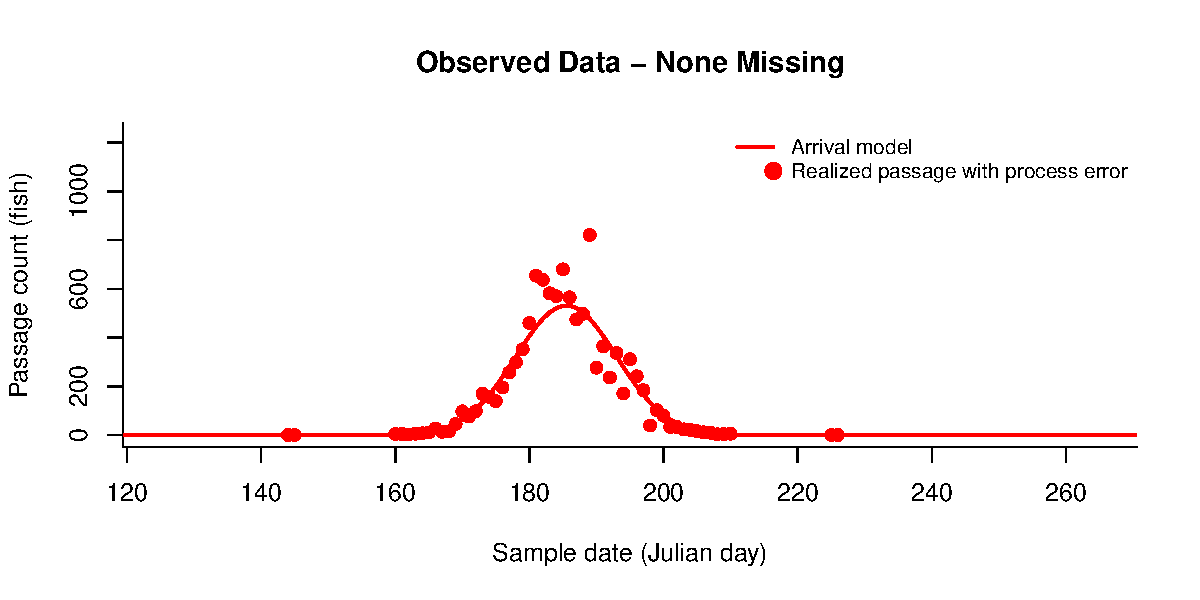
\includegraphics[width=\linewidth]{figure/plotdat-1} 

\end{knitrout}

\noindent The following code removes some of the data to represent a ``weekends off'' scenario where data are missing from the weekends. The plot below shows the data after the missing dates have been removed.

\begin{knitrout}\footnotesize
\definecolor{shadecolor}{rgb}{0.969, 0.969, 0.969}\color{fgcolor}\begin{kframe}
\begin{alltt}
\hlcom{# remove "weekend" data, i.e. sample for five days, take two off, sample five days...}
\hlstd{`%notin%`}\hlkwb{<-} \hlkwd{Negate}\hlstd{(`%in%`)} \hlcom{# helper function}
\hlstd{knockout.date.v} \hlkwb{<-} \hlstd{obs.dat.v[}\hlnum{1}\hlopt{:}\hlkwd{nrow}\hlstd{(obs.dat.v)} \hlopt
                               \hlkwd{c}\hlstd{(}\hlkwd{seq}\hlstd{(}\hlkwc{from}\hlstd{=}\hlnum{6}\hlstd{,}\hlkwc{to}\hlstd{=}\hlkwd{nrow}\hlstd{(obs.dat.v),}\hlkwc{by}\hlstd{=}\hlnum{7}\hlstd{),}
                                 \hlkwd{seq}\hlstd{(}\hlkwc{from}\hlstd{=}\hlnum{7}\hlstd{,}\hlkwc{to}\hlstd{=}\hlkwd{nrow}\hlstd{(obs.dat.v),}\hlkwc{by}\hlstd{=}\hlnum{7}\hlstd{)),} \hlstr{"Date"}\hlstd{]} \hlcom{#missed weekends}
\hlstd{knockout.passage.v} \hlkwb{<-} \hlstd{obs.dat.v[obs.dat.v}\hlopt{$}\hlstd{Date} \hlopt \hlstd{knockout.date.v,} \hlstr{"Count"}\hlstd{]} \hlcom{# missed passages}
\hlstd{obs.dat.v} \hlkwb{<-} \hlstd{obs.dat.v[obs.dat.v}\hlopt{$}\hlstd{Date} \hlopt \hlstd{knockout.date.v, ]} \hlcom{#remove weekend passages from dataset}
\end{alltt}
\end{kframe}
\end{knitrout}

\begin{knitrout}\footnotesize
\definecolor{shadecolor}{rgb}{0.969, 0.969, 0.969}\color{fgcolor}
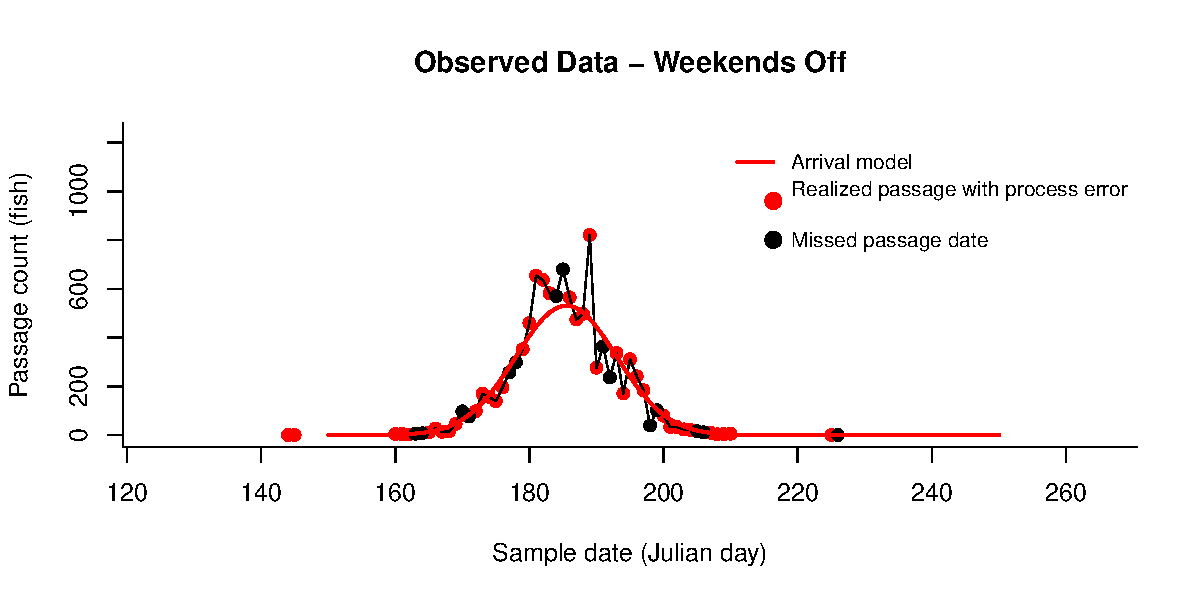
\includegraphics[width=\linewidth]{figure/plotall-1} 

\end{knitrout}

\noindent The following code removes data in the early tail of the run to represent a scenario where the weir couldn't be installed until after the run had began. The plot below shows the data with the initial $15\%$ removed.



\begin{knitrout}\footnotesize
\definecolor{shadecolor}{rgb}{0.969, 0.969, 0.969}\color{fgcolor}\begin{kframe}
\begin{alltt}
\hlcom{# remove first 15% of data}
\hlstd{`%notin%`}\hlkwb{<-} \hlkwd{Negate}\hlstd{(`%in%`)} \hlcom{# helper function}
\hlstd{knockout.date.v} \hlkwb{<-} \hlstd{obs.dat.v[}\hlnum{3}\hlopt{:}\hlnum{11}\hlstd{,} \hlstr{"Date"}\hlstd{]} \hlcom{#missed early tail}
\hlstd{knockout.passage.v} \hlkwb{<-} \hlstd{obs.dat.v[obs.dat.v}\hlopt{$}\hlstd{Date} \hlopt \hlstd{knockout.date.v,} \hlstr{"Count"}\hlstd{]} \hlcom{# missed passages (initial 15%)}
\hlstd{obs.dat.v} \hlkwb{<-} \hlstd{obs.dat.v[obs.dat.v}\hlopt{$}\hlstd{Date} \hlopt \hlstd{knockout.date.v, ]} \hlcom{#remove intial 15%}
\end{alltt}
\end{kframe}
\end{knitrout}

\begin{knitrout}\footnotesize
\definecolor{shadecolor}{rgb}{0.969, 0.969, 0.969}\color{fgcolor}
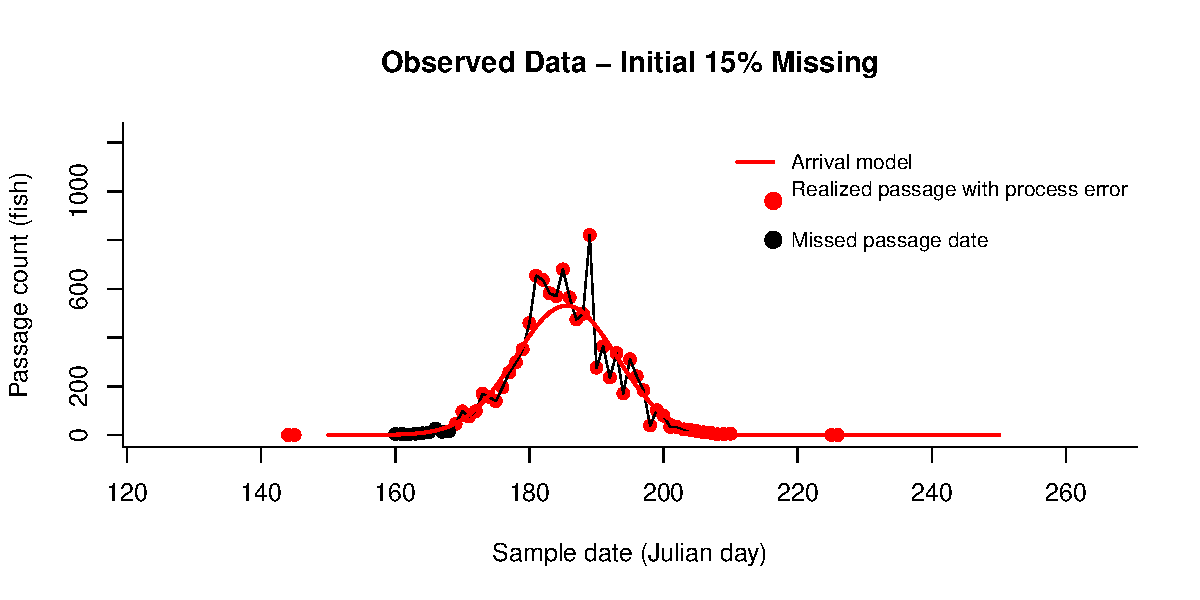
\includegraphics[width=\linewidth]{figure/plotalltail-1} 

\end{knitrout}



\section{Model fitting and results}







\section{Posterior predictive checks}

\section{My opinions and what I learned}

\section{Recommendations}



  



\section{References}


\noindent Gewin, C.S., and VanHatten, G.K. 2005. Abundance and run timing of adult Pacific Salmon in the East Fork Andreafsky River, Yukon Delta National Wildlife Refuge, Alaska, 2003. U.S. Fish and Wildlife Service Data Series Report 2005-10, Anchorage, Alaska. \\

\noindent Johnson, D.H., Shrier, B.M., O’Neal, J.S., Knutzen, J.A., Augerot, X., O’Neil, T.A., and Pearsons, T.A. (Eds.) 2007. Salmon field protocols handbook. American Fisheries Society, Bethesda, Maryland. \\

\noindent Suresh, Sethi, and Catherine Bradley. "Statistical Arrival Models to Estimate Missed Passage Counts at Fish Weirs." Canadian Journal of Fisheries and Aquatic Sciences. Draft. \\

\noindent   R Core Team (2014). R: A language and environment for statistical
computing. R Foundation for Statistical Computing, Vienna, Austria. URL
http://www.R-project.org/.\\

\section{R Code Appendix}



\end{document}



\begin{center}
\begin{knitrout}\footnotesize
\definecolor{shadecolor}{rgb}{0.969, 0.969, 0.969}\color{fgcolor}
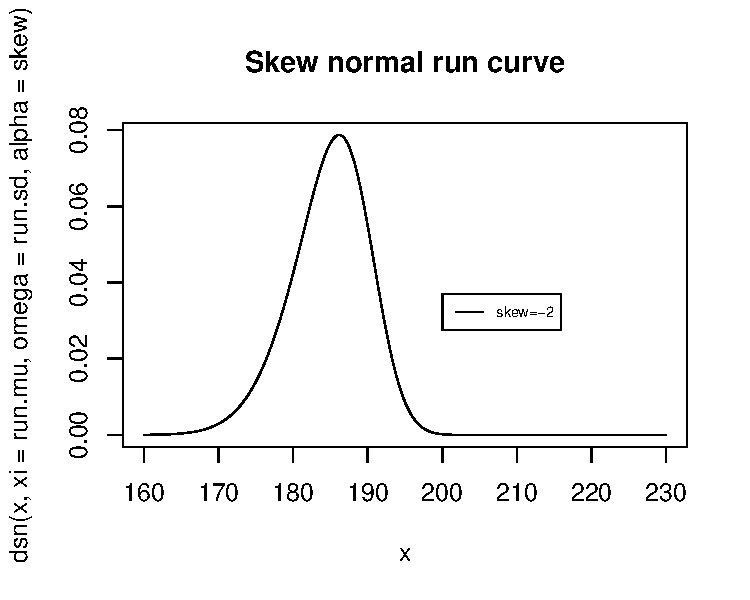
\includegraphics[width=\linewidth]{figure/dsn-1} 

\end{knitrout}
\end{center}



\begin{knitrout}\footnotesize
\definecolor{shadecolor}{rgb}{0.969, 0.969, 0.969}\color{fgcolor}
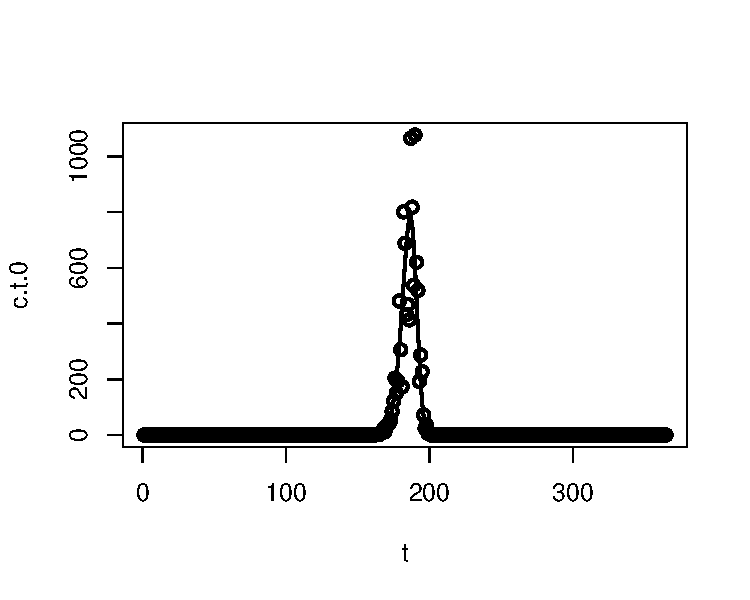
\includegraphics[width=\linewidth]{figure/processvariation-1} 

\end{knitrout}








